\documentclass[unicode,bookmarksnumbered]{beamer}

\usepackage{lmodern} % Sázet se bude Latin Modern fonty, nikoli výchozími EC
%fonty.
\usepackage[czech, english]{babel}
\usepackage[utf8]{inputenc}
\usepackage[T1]{fontenc}
%\usepackage{cmap}
\usepackage{booktabs}
\usepackage{graphicx}
\usepackage{color}
\usepackage{hyperref} 
\usepackage{listings}

%\usepackage{times}

\usetheme{Hannover}%Berlin
\usecolortheme{whale}%dolphin}

% \setbeamercovered{invisible}		%zadne - nejsou videt
% \setbeamercovered{transparent}	%jsou videt / ale jen trochu
\setbeamercovered{dynamic}		%prvni volba zvyraznena, dalsi dve tranparentni,
%postupne se zvyraznuji dalsi
% \setbeamercovered{highly dynamic}	%zvyrazneni neaktivnich casti seznamu 

% nasledujici volba zpusobi, ze vycty v~prezentaci se zobrazuji postupne
%\beamerdefaultoverlayspecification{<+->}

\usepackage{multimedia}
\title[]{Využití distribuovaných databázových systémů pro správu vektorových dat
	v GIS}
\subtitle{Diplomová práce}
\author{Matěj Krejčí} 

\institute[ČVUT]{ČESKÉ VYSOKÉ UČENÍ TECHNICKÉ V PRAZE\\
	Katedra geomatiky}

\def\denD{23.\,6.\,2016} % den prezentace
\date[červen 2016]{{\denD} }

\logo{
\includegraphics[scale=0.4]{./img/logo.pdf} }

\setbeamercolor{block title}{bg=red!40!black,fg=white}  % nastavení barvy
%definic apod.
%\setbeamercolor{block body}{bg=white,fg=black}
\setbeamercolor*{item}{fg=red!60!black}  % nastavení barvy puntíků

%zacatek dokumentu
\begin{document}
	
	\begin{frame}
		\titlepage % uvodni stranka
	\end{frame}
	
	%%%%%%%%%%%%%%%%%%%%%%%%%%%%%%%%%%%%%%%%%%%%%%%%%%%%%%%%%%%%%%%%%%%%%%%
	\section{Motivace}
	\begin{frame}
		\begin{figure}
			\frametitle{Vývoj počtu vektorových prvků v OSM History datasetu}
			\centering
			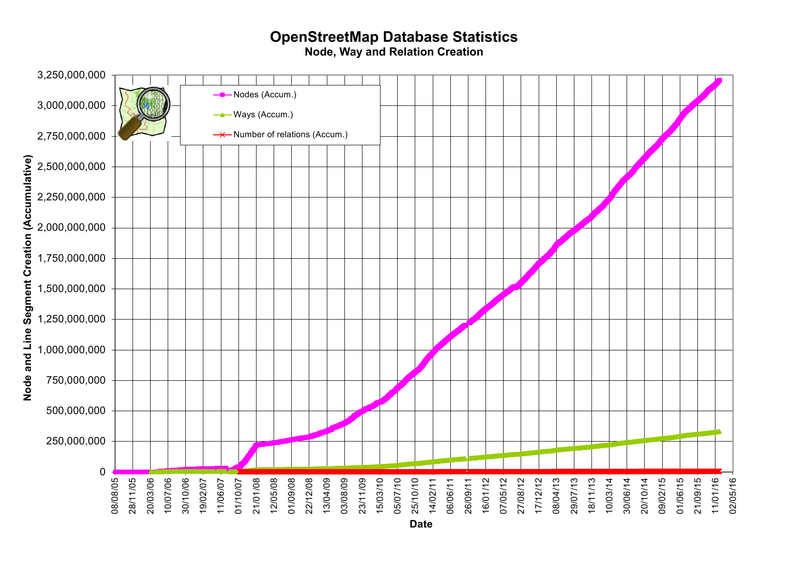
\includegraphics[width=0.9\textwidth]{./img/motivace/osm_graph.png}
			\label{fig:osm_history}
		\end{figure}
		Zdroj: OpenStreetMap Statistics
	\end{frame}
	
%%%%%%%%%%%%%%%%%%%%%%%%%%%%%%%%%%%%%%%%%%%%%%%%%%%%%%%%%%%
% dataset obsahuje 116gb = big data
% definice big data
%%%%%%%%%%%%%%%%%%%%%%%%%%%%%%%%%%%%%%%%%%%%%%%%%%%%%%%%%%%



%%%%%%%%%%%%%%%%%%%%%%%%%%%%%%%%%%%%%%%%%%%%%%%%%%%%%%%%%%%

%%%%%%%%%%%%%%%%%%%%%%%%%%%%%%%%%%%%%%%%%%%%%%%%%%%%%%%%%%%
%%%%%%%%%%%%%%%%%%%%%%%%%%%%%%%%%%%%%%%%%%%%%%%%%%%%%%%%%%%
%%%%%%%%%%%%%%%%%%%%%%%%%%%%%%%%%%%%%%%%%%%%%%%%%%%%%%%%%%%	

%%%%%%%%%%%%%%%%%%%%%%%%%%%%%%%%%%%%%%%%%%%%%%%%%%%%%%%%%%%
	\begin{frame}
		\frametitle{Vizualizace OSM History dataset pro Evropu}
		\begin{figure}
			\centering
			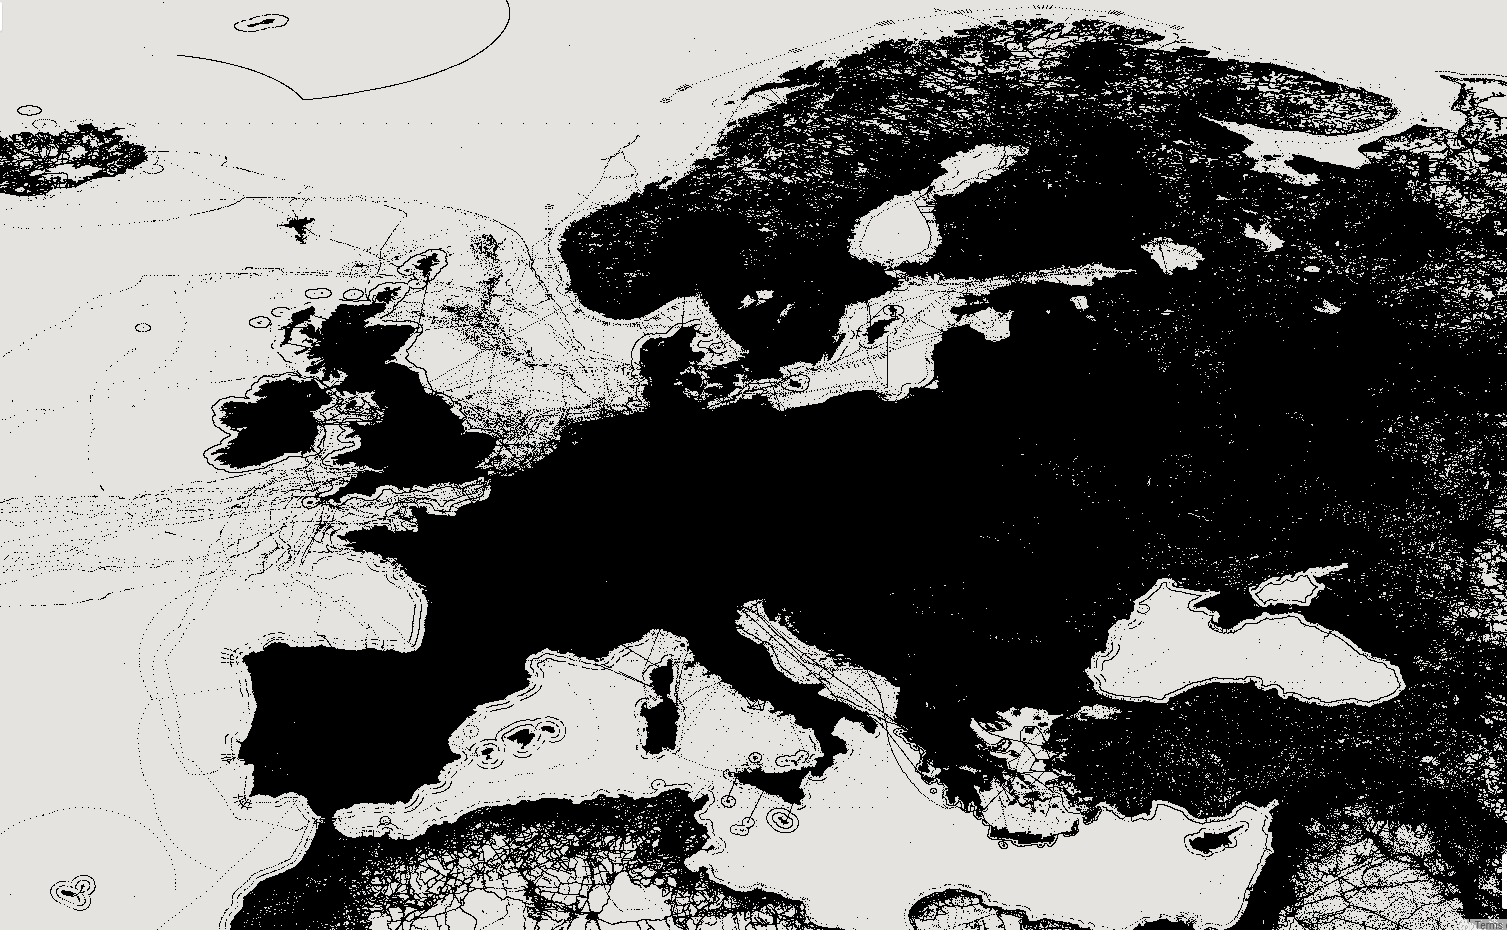
\includegraphics[width=0.9\textwidth]{./img/motivace/eu_all.png}
			\label{fig:eu_all}
		\end{figure}
		Zdroj: SpatialHadoop
	\end{frame}
%%%%%%%%%%%%%%%%%%%%%%%%%%%%%%%%%%%%%%%%%%%%%%%%%%%%%%%%%%%
% jak vypada vizualizace bodu
% bez vizualizace nelze jednoduse videt informaci
% bez processing nelze visualisovat
%%%%%%%%%%%%%%%%%%%%%%%%%%%%%%%%%%%%%%%%%%%%%%%%%%%%%%%%%%%
%%%%%%%%%%%%%%%%%%%%%%%%%%%%%%%%%%%%%%%%%%%%%%%%%%%%%%%%%%%

%%%%%%%%%%%%%%%%%%%%%%%%%%%%%%%%%%%%%%%%%%%%%%%%%%%%%%%%%%%
	\begin{frame}
		\frametitle{Desktopové GIS}
		\begin{figure}
			\centering
			
\includegraphics[width=1\textwidth]{./img/motivace/no.png}
			\label{fig:eu_all}
		\end{figure}
	\end{frame}
%%%%%%%%%%%%%%%%%%%%%%%%%%%%%%%%%%%%%%%%%%%%%%%%%%%%%%%%%%%
% standardni desktop gis nestaci
% trva to dlouho
%%%%%%%%%%%%%%%%%%%%%%%%%%%%%%%%%%%%%%%%%%%%%%%%%%%%%%%%%%%
%%%%%%%%%%%%%%%%%%%%%%%%%%%%%%%%%%%%%%%%%%%%%%%%%%%%%%%%%%%

%%%%%%%%%%%%%%%%%%%%%%%%%%%%%%%%%%%%%%%%%%%%%%%%%%%%%%%%%%%
	\begin{frame}
		\frametitle{GIS pro distribuované systémy - Hadoop}
		\begin{figure}
			\centering
			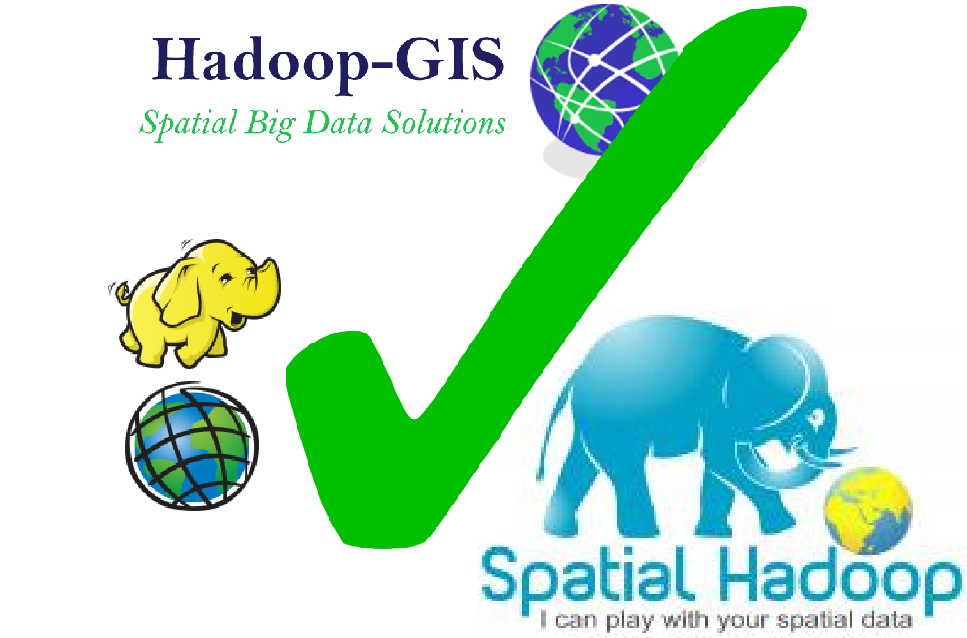
\includegraphics[width=1\textwidth]{./img/motivace/yes.png}
			\label{fig:eu_all}
		\end{figure}
	\end{frame}
%%%%%%%%%%%%%%%%%%%%%%%%%%%%%%%%%%%%%%%%%%%%%%%%%%%%%%%%%%%
%
%%%%%%%%%%%%%%%%%%%%%%%%%%%%%%%%%%%%%%%%%%%%%%%%%%%%%%%%%%%
%%%%%%%%%%%%%%%%%%%%%%%%%%%%%%%%%%%%%%%%%%%%%%%%%%%%%%%%%%%
	\begin{frame}
		\begin{figure}
			\frametitle{Počet publikací v databázi ResearchGate s klíčovým slovem BigData}
			\centering
			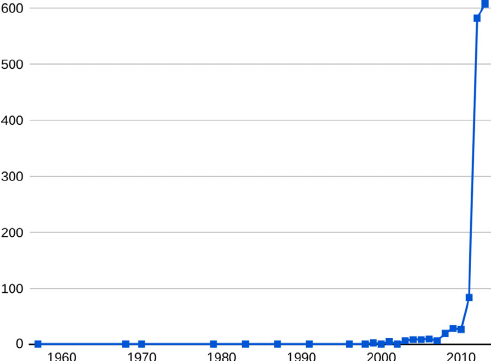
\includegraphics[width=0.8\textwidth]{./img/motivace/num_of_publication.png}
			\label{fig:num_of_publication}
		\end{figure}
		Zdroj: ResearchGate
	\end{frame}
%%%%%%%%%%%%%%%%%%%%%%%%%%%%%%%%%%%%%%%%%%%%%%%%%%%%%%%%%%%
%
%%%%%%%%%%%%%%%%%%%%%%%%%%%%%%%%%%%%%%%%%%%%%%%%%%%%%%%%%%%
%%%%%%%%%%%%%%%%%%%%%%%%%%%%%%%%%%%%%%%%%%%%%%%%%%%%%%%%%%%

	%\begin{frame}
	%	\begin{figure}
	%		\frametitle{Odhad vývoje trhu v souvislosti s Big Data a Hadoop }
	%		\centering
	%		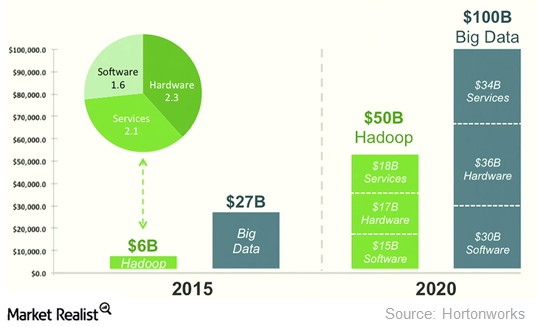
\includegraphics[width=0.9\textwidth]{./img/motivace/hadoop_market.png}
	%		\label{fig:hadoop_market}
	%	\end{figure}
	%	Zdroj: Hortonworks
	%\end{frame}
%%%%%%%%%%%%%%%%%%%%%%%%%%%%%%%%%%%%%%%%%%%%%%%%%%%%%%%%%%%
%
%%%%%%%%%%%%%%%%%%%%%%%%%%%%%%%%%%%%%%%%%%%%%%%%%%%%%%%%%%%
%%%%%%%%%%%%%%%%%%%%%%%%%%%%%%%%%%%%%%%%%%%%%%%%%%%%%%%%%%%

	\section{Úvod}  % říct zadání a~cíle práce
	\begin{frame}
		\frametitle{Zadání}
Diplomová práce se věnuje analýze technologií pro zpracování velkého množství dat (tzv. bigdata). Konktrétně je zaměřena na uložení a správu časoprostorových vektorových dat v prostředí distribuovaných databázových systémů jako je např. Hadoop. Cílem praktické části práce je jejich zpřístupnění a umožnění analýz v prostředí desktopového open source GIS nástroje GRASS GIS. Testování navrženého řešení bude prováděno s využitím virtualizované sítě uzlů tvořících cluster.

	\end{frame}
%%%%%%%%%%%%%%%%%%%%%%%%%%%%%%%%%%%%%%%%%%%%%%%%%%%%%%%%%%%
%
%%%%%%%%%%%%%%%%%%%%%%%%%%%%%%%%%%%%%%%%%%%%%%%%%%%%%%%%%%%
%%%%%%%%%%%%%%%%%%%%%%%%%%%%%%%%%%%%%%%%%%%%%%%%%%%%%%%%%%%

	\begin{frame}
		\frametitle{Řešení}
		Návrh postupu pro zpracování objemných vektorových datasetů z prostředí GIS
		\begin{itemize}
			\item Teoretický základ Hadoop a jeho GIS extenzí
			\item Konfigurace Hadoop clusteru hostovaného na Google Cloud Platform
			\item Vývoj GRASS Hadoop Framework umožňující interakci desktop GIS s Hadoop/Hive a jeho GIS exetenzemi
			\item Otestovaní navrženého workflow
		\end{itemize}
		
\includegraphics[width=0.5\textwidth]{./img/motivace/zadani.jpg}
	\end{frame}
%%%%%%%%%%%%%%%%%%%%%%%%%%%%%%%%%%%%%%%%%%%%%%%%%%%%%%%%%%%
%
%%%%%%%%%%%%%%%%%%%%%%%%%%%%%%%%%%%%%%%%%%%%%%%%%%%%%%%%%%%
%%%%%%%%%%%%%%%%%%%%%%%%%%%%%%%%%%%%%%%%%%%%%%%%%%%%%%%%%%%


	\begin{frame}
		\frametitle{Struktura prezentace}
		\begin{itemize}
			\item Úvod do Hadoop 
			\item GIS extenze pro Hadoop
			\item Hadoop konfigurací a cloudové služby
			\item Seznámení s vyvinutým software
			\item Případová studie
			\item Závěr
		\end{itemize}
	\end{frame}
%%%%%%%%%%%%%%%%%%%%%%%%%%%%%%%%%%%%%%%%%%%%%%%%%%%%%%%%%%%
%
%%%%%%%%%%%%%%%%%%%%%%%%%%%%%%%%%%%%%%%%%%%%%%%%%%%%%%%%%%%
%%%%%%%%%%%%%%%%%%%%%%%%%%%%%%%%%%%%%%%%%%%%%%%%%%%%%%%%%%%


	\section{Hadoop}
	\begin{frame}[c]
		\begin{center}	
		\Huge Hadoop - teoretický základ
		\end{center}
	\end{frame}
 
	\begin{frame}
		\frametitle{Hadoop Framework}

			\begin{itemize}
				\item Sada \textbf{open-source} komponent pro zpracování velkého množství.
dat v řádech petabytů a exabytů.  
				\item Uložení a zpracování objemných dat na velkém množství běžných počítačů. 
				\item Dvě hlavní komponenty:
				\begin{enumerate}
					\item distribuovaný file systém, nativně \textbf{HDFS},
					\item framework \textbf{MapReduce} pro paralelní výpočy.
				\end{enumerate}
			\end{itemize}
			\begin{figure}
				\centering
				
\includegraphics[width=0.4\textwidth]{./img/hadoop/hadoop_logo.jpg}
			\end{figure}
	\end{frame}
%%%%%%%%%%%%%%%%%%%%%%%%%%%%%%%%%%%%%%%%%%%%%%%%%%%%%%%%%%%
%
%%%%%%%%%%%%%%%%%%%%%%%%%%%%%%%%%%%%%%%%%%%%%%%%%%%%%%%%%%%
%%%%%%%%%%%%%%%%%%%%%%%%%%%%%%%%%%%%%%%%%%%%%%%%%%%%%%%%%%%


	\begin{frame}
		\frametitle{Hadoop Framework - komponenty}
		\textbf{Dvě hlavní komponenty - HDFS a MapReduce}
		\begin{figure}
			\centering
			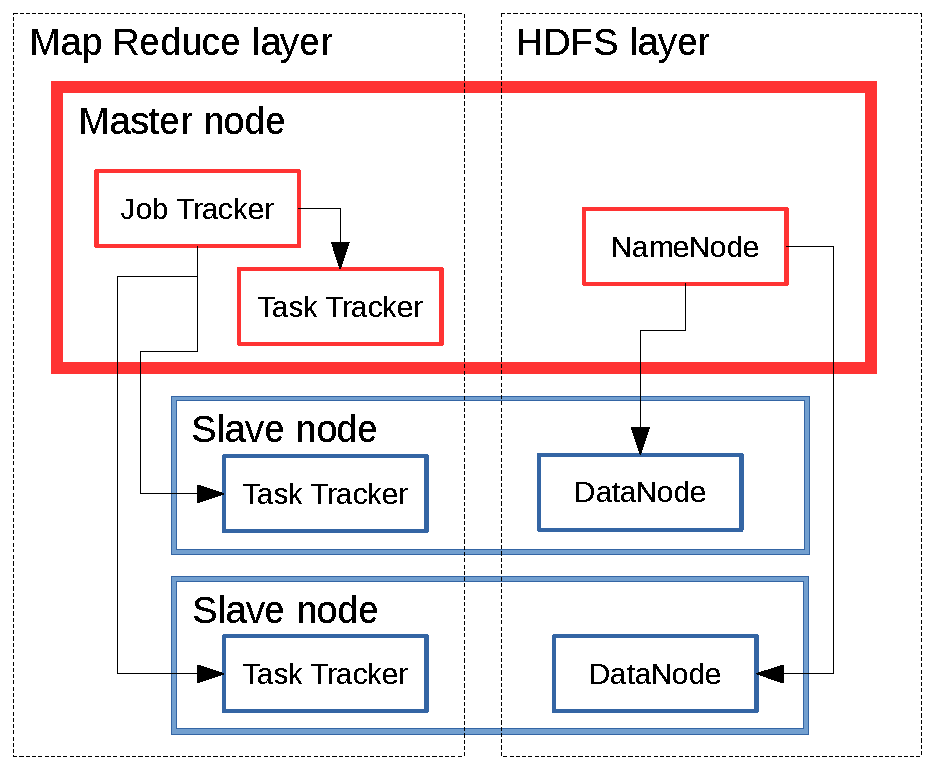
\includegraphics[width=0.7\textwidth]{./img/hadoop/schema2.pdf}
		\end{figure}
	\end{frame}
%%%%%%%%%%%%%%%%%%%%%%%%%%%%%%%%%%%%%%%%%%%%%%%%%%%%%%%%%%%%%%%%%%%%%%%
	\subsection{HDFS} 
	\begin{frame}
		\frametitle{Hadoop Distributed File System}  
			\textbf{Serverové komponenty HDFS}
			\begin{itemize}
				\item \textbf{NameNode} - \textbf{master} - Udržuje metadata filesystému.
				\item \textbf{DataNode} - \textbf{slave} -  Jsou instalovány na každém uzlu
a disponují data bloky. Zajišťují čtení a zápis dat od klienta.
				\item \textbf{Secondary NameNode} - periodicky zajišťuje zálohu metadata
logů. V případě selhání NameNode umožňuje obnovu z poslední zálohy.
			\end{itemize}
		\begin{figure}
			\centering
			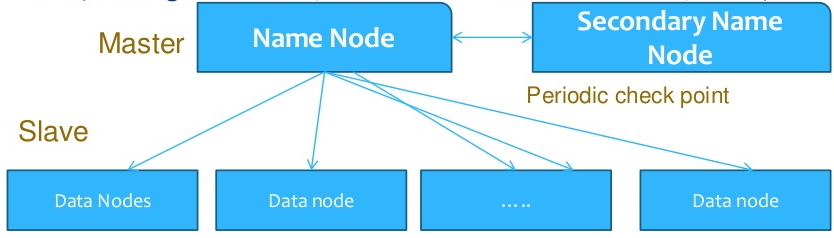
\includegraphics[width=0.7\textwidth]{./img/hadoop/ms.png}
		\end{figure}
	\end{frame}
%%%%%%%%%%%%%%%%%%%%%%%%%%%%%%%%%%%%%%%%%%%%%%%%%%%%%%%%%%%
%
%%%%%%%%%%%%%%%%%%%%%%%%%%%%%%%%%%%%%%%%%%%%%%%%%%%%%%%%%%%
%%%%%%%%%%%%%%%%%%%%%%%%%%%%%%%%%%%%%%%%%%%%%%%%%%%%%%%%%%%


	\begin{frame}
		\frametitle{Distribuovaný file systém}
		\textbf{Hlavní vlastnosti}
		\begin{itemize}
			\item abstraktní vrstva - umožňuje využití jiných file systémů
			\begin{itemize}
				\item 		Nativní distribuovaný file systém - \textbf{Hadoop Distributed File System(HDFS)}
			\end{itemize}
			\item škálovatelnost 
			\item replikace ->fault tolerant
			\item vysoká propustonst dat
		\end{itemize}

	\end{frame}
%%%%%%%%%%%%%%%%%%%%%%%%%%%%%%%%%%%%%%%%%%%%%%%%%%%%%%%%%%%
%
%%%%%%%%%%%%%%%%%%%%%%%%%%%%%%%%%%%%%%%%%%%%%%%%%%%%%%%%%%%
%%%%%%%%%%%%%%%%%%%%%%%%%%%%%%%%%%%%%%%%%%%%%%%%%%%%%%%%%%%


%	\begin{frame}
%		\frametitle{Hadoop Distributed File System}  
%		\textbf{Data bloky}
%		\begin{figure}
%			\centering
%			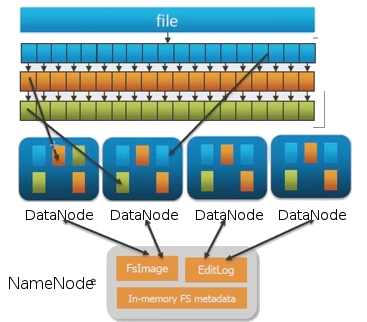
\includegraphics[width=0.7\textwidth]{./img/hadoop/block1.png}
%		\end{figure}
%		Zdroj: edureka.co
%	\end{frame}
%%%%%%%%%%%%%%%%%%%%%%%%%%%%%%%%%%%%%%%%%%%%%%%%%%%%%%%%%%%
%
%%%%%%%%%%%%%%%%%%%%%%%%%%%%%%%%%%%%%%%%%%%%%%%%%%%%%%%%%%%
%%%%%%%%%%%%%%%%%%%%%%%%%%%%%%%%%%%%%%%%%%%%%%%%%%%%%%%%%%%


	\subsection{MapReduce} 
	\begin{frame}
		\frametitle{MapReduce} 
		Programovací model pro paralelní zpracování velkého objemu dat s využitím
počítačévého clusteru.
		
		Princip MapReduce   
		\begin{enumerate}
			\item \textbf{Map} fáze - Každý \textbf{Slave} počítač zavolá funkci
\textit{Map()} nad lokálními daty a dočasně zapíše mezivýsledky. Master počítač
zajišťuje, že je zpracována pouze jedna replika.
			%\item  \textbf{Shuffle} fáze - \textbf{Slave} předistribujuje mezivísledky
%fce. map() tak, aby \textit{value} každého \textit{key} byla na stejném Slave
%počítači.			
			\item \textbf{Reduce} fáze - Slave počítače paralelně zpracují jednotlivé
skupiny key-value pomocí uživatelem definované funkce Reduce()
		\end{enumerate}
	\end{frame}
%%%%%%%%%%%%%%%%%%%%%%%%%%%%%%%%%%%%%%%%%%%%%%%%%%%%%%%%%%%
%
%%%%%%%%%%%%%%%%%%%%%%%%%%%%%%%%%%%%%%%%%%%%%%%%%%%%%%%%%%%
%%%%%%%%%%%%%%%%%%%%%%%%%%%%%%%%%%%%%%%%%%%%%%%%%%%%%%%%%%%


	\begin{frame}
		\frametitle{MapReduce}
		Četnost slov
		\begin{figure}
			\centering
			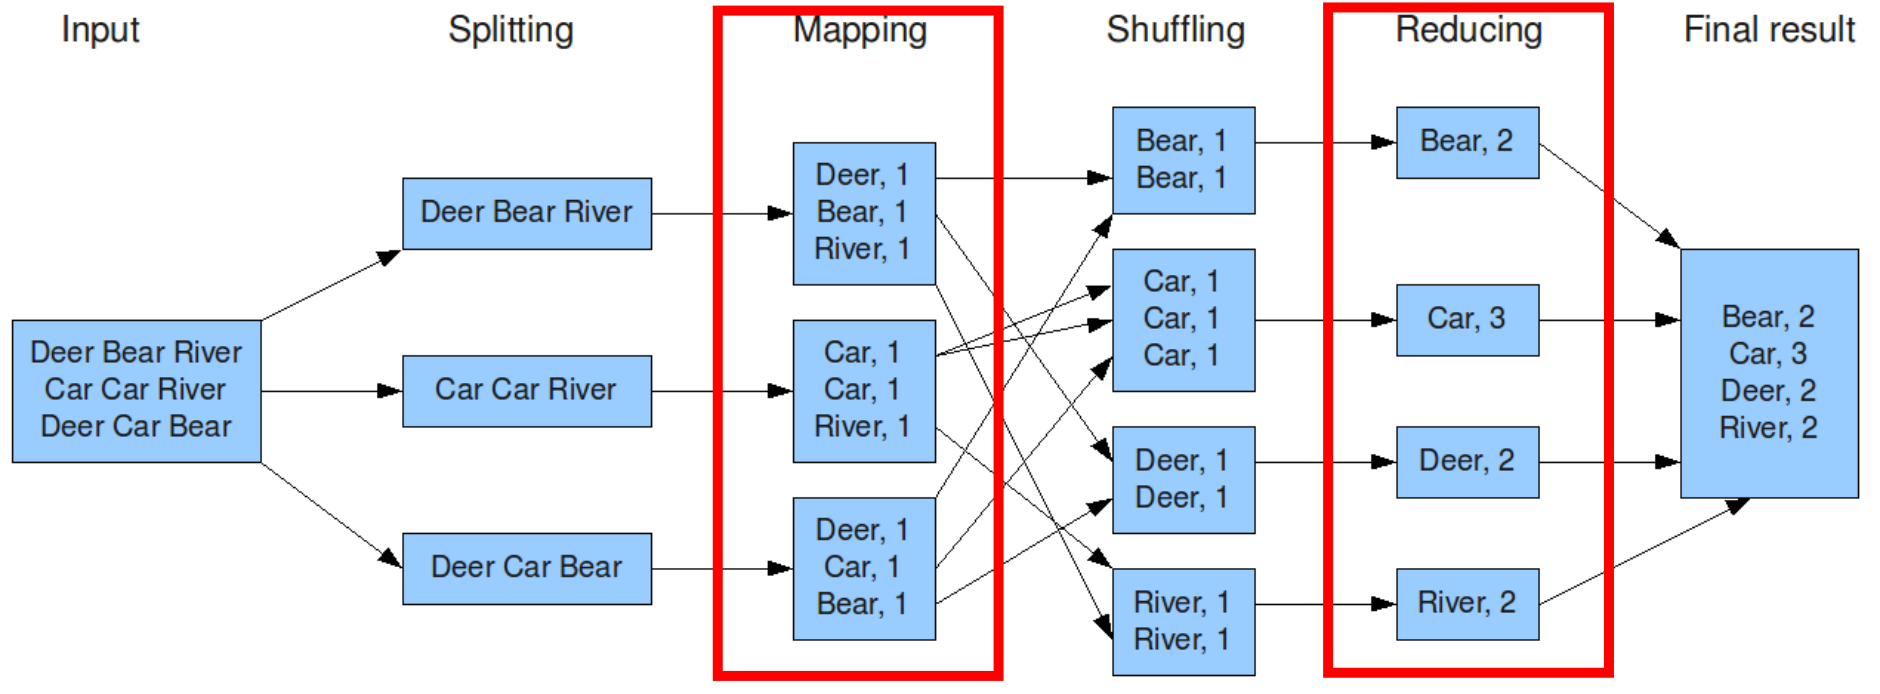
\includegraphics[width=1\textwidth]{./img/hadoop/maprede.png}
			\label{fig:eu_all}
		\end{figure}
	\end{frame}
%%%%%%%%%%%%%%%%%%%%%%%%%%%%%%%%%%%%%%%%%%%%%%%%%%%%%%%%%%%
%
%%%%%%%%%%%%%%%%%%%%%%%%%%%%%%%%%%%%%%%%%%%%%%%%%%%%%%%%%%%
%%%%%%%%%%%%%%%%%%%%%%%%%%%%%%%%%%%%%%%%%%%%%%%%%%%%%%%%%%%


	%\begin{frame}
	%	\frametitle{MapReduce}  
	%	\textbf{TODO}
	%	\begin{itemize}
	%		\item \textbf{JobTracker} 
	%		\item \textbf{TasksTrackers} 
	%	\end{itemize}
	%	\begin{figure}
			%\centering
			%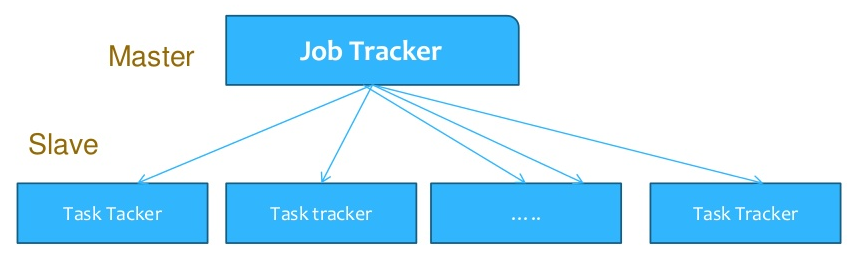
\includegraphics[width=0.7\textwidth]{./%img/hadoop/ms1.png}
	%	\end{figure}
	%\end{frame}

%%%%%%%%%%%%%%%%%%%%%%%%%%%%%%%%%%%%%%%%%%%%%%%%%%%%%%%%%%%%%%%%%%%%%%%
	\section{GIS Hadoop}
	\begin{frame}[c]
		\begin{center}	
		\Huge GIS vektorové analýzy paralelně
		\end{center}
	\end{frame}
	
	
		\subsection{GIS Extenze}
		\begin{frame}
			\frametitle{GIS extenze pro Hadoop}
		Pro MapReduce framework jsou dostupné extenze, které podporují základní GIS
operace nad prostorovými daty. Analogií v relačních databázích je PostGIS
pro PostgreSQL.
			\begin{enumerate}
				\item Esri Spatial processing framework for Hadoop
				\item HadoopGIS
				\item SpatialHadoop
			\end{enumerate}
		\end{frame}
%%%%%%%%%%%%%%%%%%%%%%%%%%%%%%%%%%%%%%%%%%%%%%%%%%%%%%%%%%%
%
%%%%%%%%%%%%%%%%%%%%%%%%%%%%%%%%%%%%%%%%%%%%%%%%%%%%%%%%%%%
%%%%%%%%%%%%%%%%%%%%%%%%%%%%%%%%%%%%%%%%%%%%%%%%%%%%%%%%%%%


	\subsection{MapReduce}
	\begin{frame}
	\frametitle{GIS MapReduce}
		\begin{figure}
			\centering
			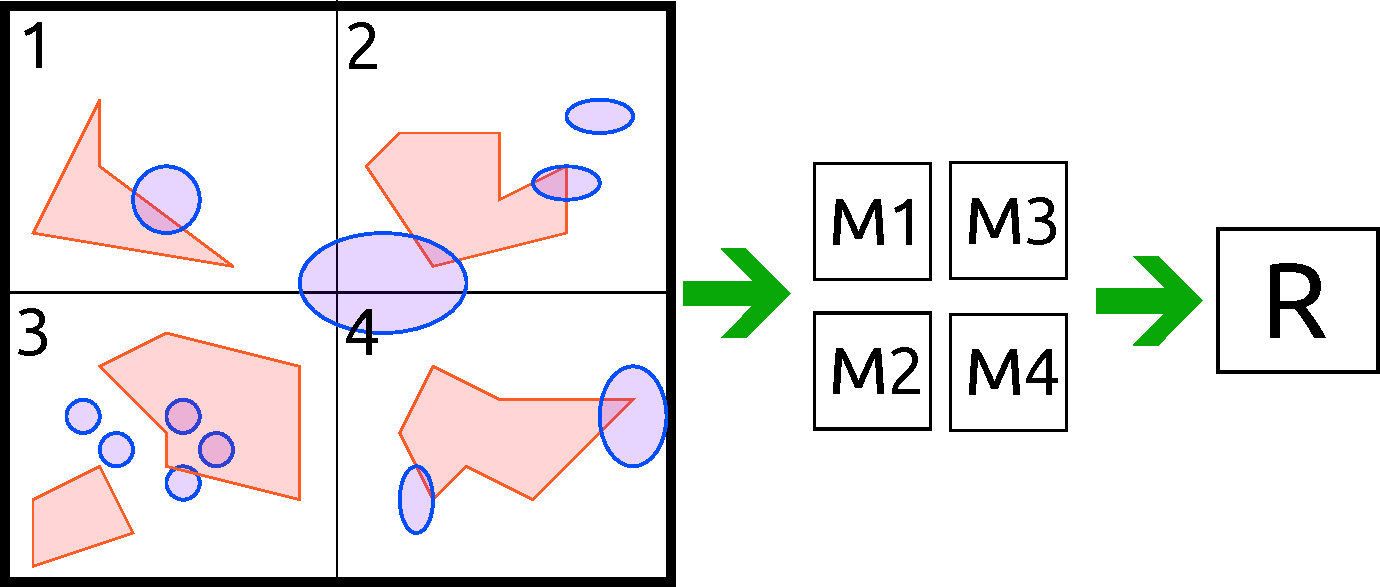
\includegraphics[width=0.8\textwidth]{./img/spatial/mapred_spatial.pdf}
		\end{figure}
		Analýza prostorového vztahu dvou datasetů.
		
		\begin{enumerate}
			\item Filtering 
			\item Partitioning
			\item Indexing
		\end{enumerate}
	\end{frame}
%%%%%%%%%%%%%%%%%%%%%%%%%%%%%%%%%%%%%%%%%%%%%%%%%%%%%%%%%%%
%
%%%%%%%%%%%%%%%%%%%%%%%%%%%%%%%%%%%%%%%%%%%%%%%%%%%%%%%%%%%
%%%%%%%%%%%%%%%%%%%%%%%%%%%%%%%%%%%%%%%%%%%%%%%%%%%%%%%%%%%


	
	\subsection{Partitioning a Indexing}
	\begin{frame}
	\frametitle{Partitioning a Indexing}
			Grid partitioning a R-tree partitioning 
			\begin{figure}
				\centering
				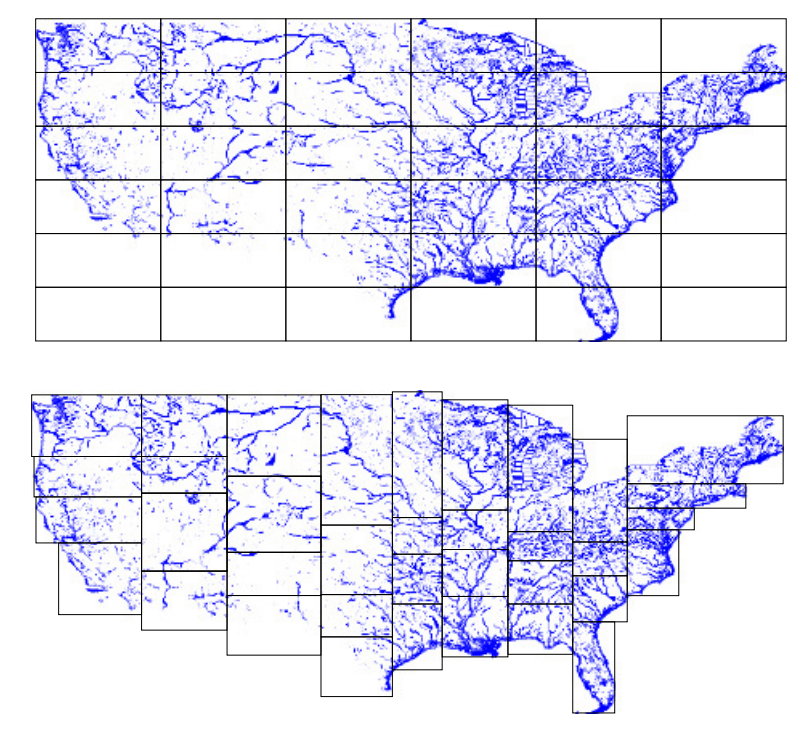
\includegraphics[width=0.8\textwidth]{./img/spatial/spatial_hadoop_parti.png}
			\end{figure}
			%\item Data skew
			%\item Hraniční objekt (Boundary Object)
	\end{frame}
%%%%%%%%%%%%%%%%%%%%%%%%%%%%%%%%%%%%%%%%%%%%%%%%%%%%%%%%%%%
%
%%%%%%%%%%%%%%%%%%%%%%%%%%%%%%%%%%%%%%%%%%%%%%%%%%%%%%%%%%%
%%%%%%%%%%%%%%%%%%%%%%%%%%%%%%%%%%%%%%%%%%%%%%%%%%%%%%%%%%%


%	\begin{frame}
%	\frametitle{Partitioning a Indexing}
	%	QuadTree pro Hadoop
	%	\begin{figure}
	%		\centering
	%		\includegraphics[width=0.6\textwidth]{./img/spatial/%esri_quad.png}
%		\end{figure}
%	\end{frame}
%%%%%%%%%%%%%%%%%%%%%%%%%%%%%%%%%%%%%%%%%%%%%%%%%%%%%%%%%%%
%
%%%%%%%%%%%%%%%%%%%%%%%%%%%%%%%%%%%%%%%%%%%%%%%%%%%%%%%%%%%
%%%%%%%%%%%%%%%%%%%%%%%%%%%%%%%%%%%%%%%%%%%%%%%%%%%%%%%%%%%


%	\begin{frame}
%		\frametitle{Funkce}
%		Základní skupiny GIS funkcí a jejich příklady:
%		\begin{enumerate}
%			\item Konstruktory - GeomFromJSON, Point, Line
%			\item Vztahy mezi vektory - Contains, Intersects
%			\item Operace - BinEnvelope, Buffer
%			\item Acesory - Distance, Centroid
%		\end{enumerate}
%	\end{frame}
%%%%%%%%%%%%%%%%%%%%%%%%%%%%%%%%%%%%%%%%%%%%%%%%%%%%%%%%%%%
%
%%%%%%%%%%%%%%%%%%%%%%%%%%%%%%%%%%%%%%%%%%%%%%%%%%%%%%%%%%%
%%%%%%%%%%%%%%%%%%%%%%%%%%%%%%%%%%%%%%%%%%%%%%%%%%%%%%%%%%%


	\subsection{Hive}
	\begin{frame}
		\frametitle{Hive}
		Co je Hive? Hadoop nadstavba, která umožňuje optimální správu dat s
expresivním dotazováním jako SQL.
				\begin{figure}
					\centering
					
\includegraphics[width=0.2\textwidth]{./img/spatial/hive.png}
				\end{figure}
		\begin{enumerate}
			\item Podpora indexů.
			\item Podpora formátů pro uložení dat - text, RCFile, HBase, ORC a další.
			\item Úložiště pro metadata je v externí RDBMS (default Derby databáze).
			\item UDFs - funkce definované uživatelem např. BinEnvelope, Intersects.
			\item SQL-like query, které jsou implicitně konvertovány do MapReduce funckcí.
		\end{enumerate}
	\end{frame}

	
	\section{Hadoop Hosting}
	\begin{frame}[c]
		\begin{center}	
		\Huge Hadoop - konfigurace a cloud služby
		\end{center}
	\end{frame}
	
	
	\subsection{Google Cloud Platform}
	\begin{frame}
		\frametitle{Konfigurace Hadoop a cloud}
		Konfigurace Hadoop serveru, Google Cloud a localhost
		\begin{enumerate}
		\item Konfigurace Google Cloud Platform prostředí
		\item Konfigurace Hadoop serveru
		\item Konfigurace počítačové sítě a firewall
		\item Konfigurace lokálního počítače
		\end{enumerate}
	\end{frame}
	
	\section{GHF}
	\begin{frame}[c]
		\begin{center}	
		\Huge Vývoj software - GRASS Hadoop Framework
		\end{center}
	\end{frame}
	\subsection{Funkcionalita}
	\begin{frame}
		\frametitle{GRASS Hadoop Framework - Úvod}
		GRASS Hadoop Framework(GHF) je sada nástrojů umožňující interakci GRASSu s Hadoop/Hive a správu uživatelských připojení. 
		
		\begin{figure}
			\centering
			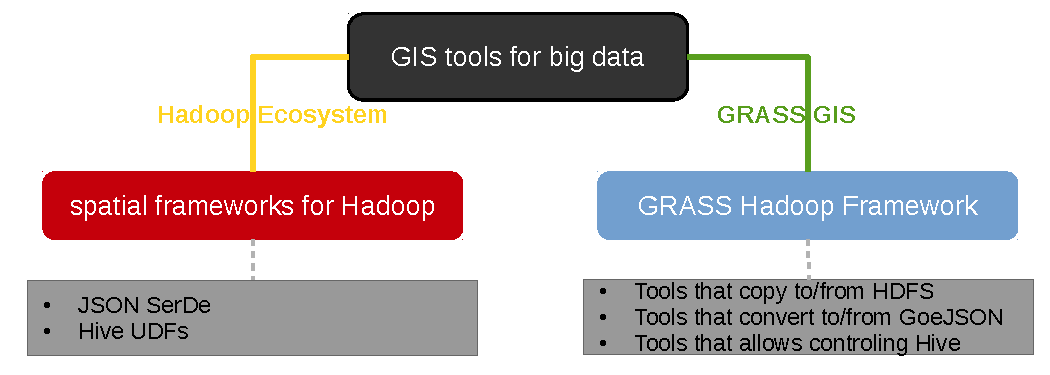
\includegraphics[width=1\textwidth]{./img/ghf/idea_schema.pdf}
		\end{figure}
	\end{frame}
	
	
%		\begin{frame}
%				\frametitle{Moduly GHF a jejich popis}
%			\begin{table}[!htbp]
%				\centering
%%				\begin{scriptsize}
%					\begin{tabular}{@{}|l|l|@{}}
%						\toprule
%						hd.hdfs.* modules  & description                    
%						\\ \midrule \midrule
%						hd.hdfs.db.connect & Management of connections     
%						table for GeoJSON  \\ \midrule
%%						hd.hdfs.in.fs      & Put data to HDFS from local      
%						table for csv data \\ \midrule
%						hd.hdfs.in.vector  & Put GRASS vectors to HDFS     
%						Hive command      \\ \midrule
%						hd.hdfs.out.vector & Put vectors from HDFS to GRASS
%						Hive query        \\ \midrule
%						hd.hdfs.info       & HDFS metadata                 
%						metadata             \\ \bottomrule
%					\end{tabular}%
%%				\end{scriptsize}
%			\end{table}
			
			
%			\begin{table}[!htbp]
%				\centering
%				\begin{scriptsize}
%					\begin{tabular}{@{}|l|l|@{}}
%						\toprule
%						 hd.hive.* modules  & description
%						\\ \midrule \midrule
%						 hd.hive.json.table & Create
%						table for GeoJSON  \\ \midrule
%						 hd.hive.csv.table  & Create
%						table for csv data \\ \midrule
%						 hd.hive.execute    & Execute
%						Hive command      \\ \midrule
%						 hd.hive.select     & Execute
%						Hive query        \\ \midrule   
%						 hd.hive.info       & Hive
%						metadata             \\ \bottomrule
%					\end{tabular}%
%				\end{scriptsize}
%			\end{table}
			
	%		
%		\end{frame}
			%\item Manager účtů pro připojení k Hadoop/Hive (SQL backend).
			%\item Konverze GRASS vektorových map do serializovatelného GeoJSON/ESRI GeoJSON.
			%\item Deserializace ESRI GeoJSON a konverze do nativních GRASS vektorových map.
			%\item PUT/GET data do Hadoop.
			%\item Vytváření Hive tabulek pro GeoJSON a CSV data.
			%\item Moduly pro Execute, Load data a Query data.

	\begin{frame}
		\frametitle{GRASS Hadoop Framework - Funkce}
		\begin{figure}
			\centering
			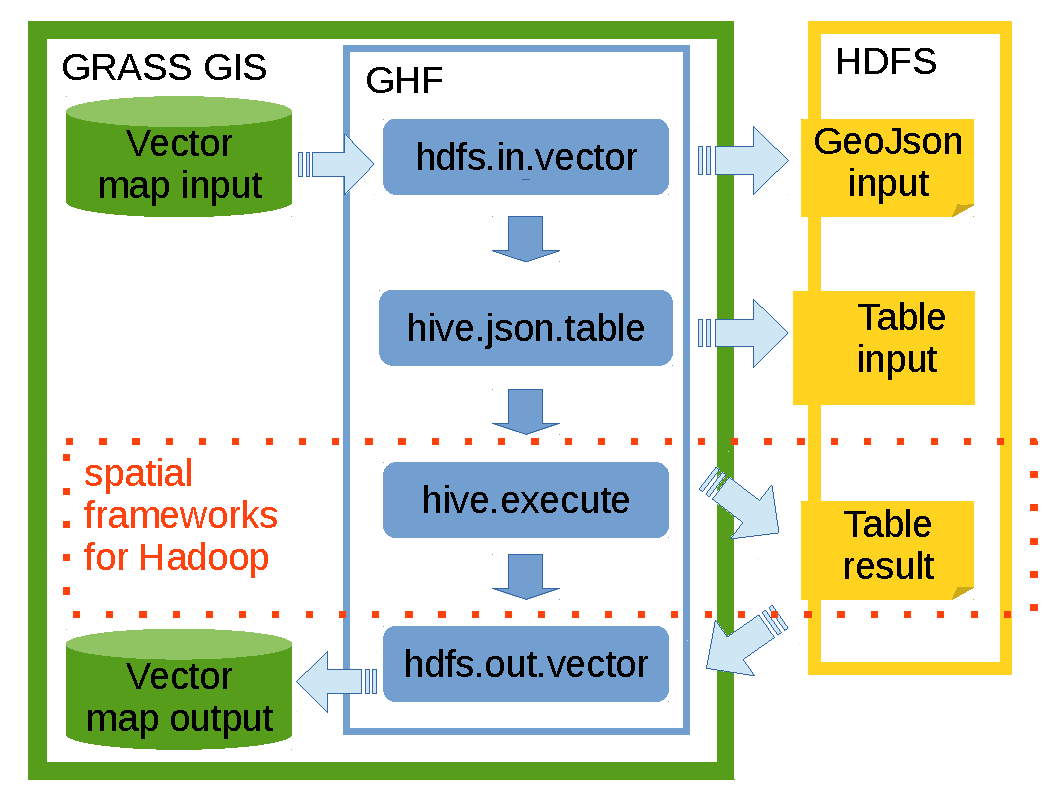
\includegraphics[width=1\textwidth]{./img/ghf/modules_schema.pdf}
		\end{figure}
	\end{frame}



%	\subsection{Implementace}
%		\begin{frame}
%			\frametitle{GRASS Hadoop Framework - Implementace}
%			Objektový návrh  dělí třidy do tří vrstev, které jsou %závislé pouze hierarchicky a s kontaktní vrstvou.
%			\begin{enumerate}
%			\item GHF core
%			\item Middle interface 
%			\item User interface
%			\end{enumerate}
	%	\end{frame}
		
		\begin{frame}
			\frametitle{GRASS Hadoop Framework - Implementace}
			\centering
			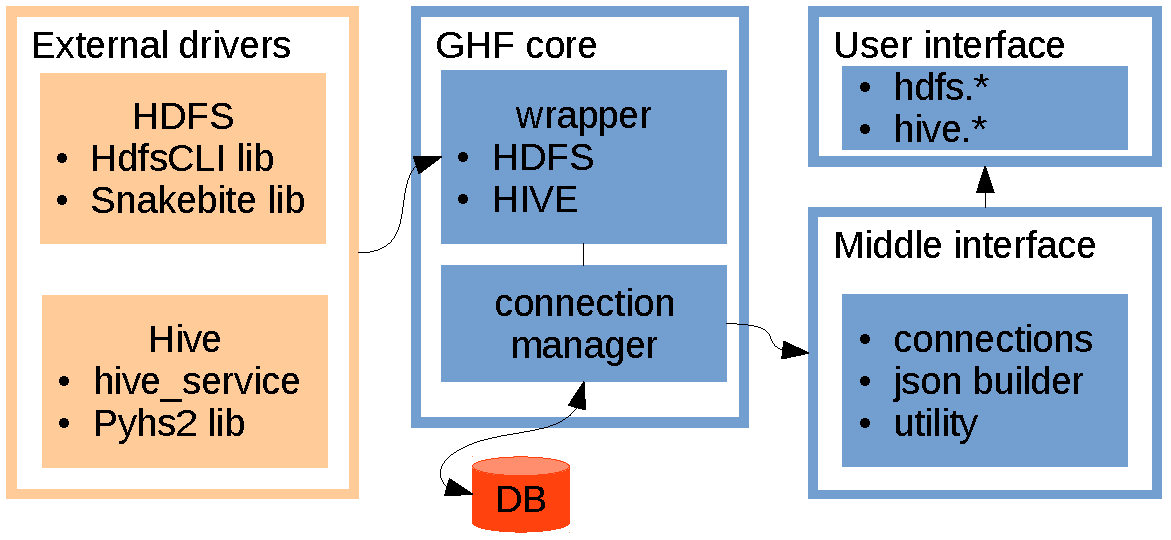
\includegraphics[width=1\textwidth]{./img/ghf/implementation.pdf}
		\end{frame}
	
	
	\subsection{Využití}
			\begin{frame}
				\frametitle{GRASS Hadoop Framework - Ovládání}
				Ovládání modulů:
			
				\begin{itemize}
					\item  z příkazové řádky GRASSu = parametry a přepínače
					\item  z vygenerovaného GUI GRASSu
				\end{itemize}
				
				%TODO obrazek gui a radky
			\end{frame}
			
	\subsection{Případová studie}		
		\begin{frame}
			\frametitle{Případová studie GHF - OSM History dataset}
			Informace o datasetu:
			\begin{itemize}
				\item  Obsahuje veškeré změny prostorových informací od založení projektu
				\item  Extrakce Evropy obsahuje cca 1.3 miliardy bodů, tj. 116 Gb
			\end{itemize}
			S využitím \textit{binning} funkce byly body z OSM agregovány do bin (obdelníků) o velikosti 0.1 stupně, tj. cca 10km.
		\end{frame}	
			
		\begin{frame}
			\frametitle{Vizualizace 1.3 miliardy bodů}
			\centering
			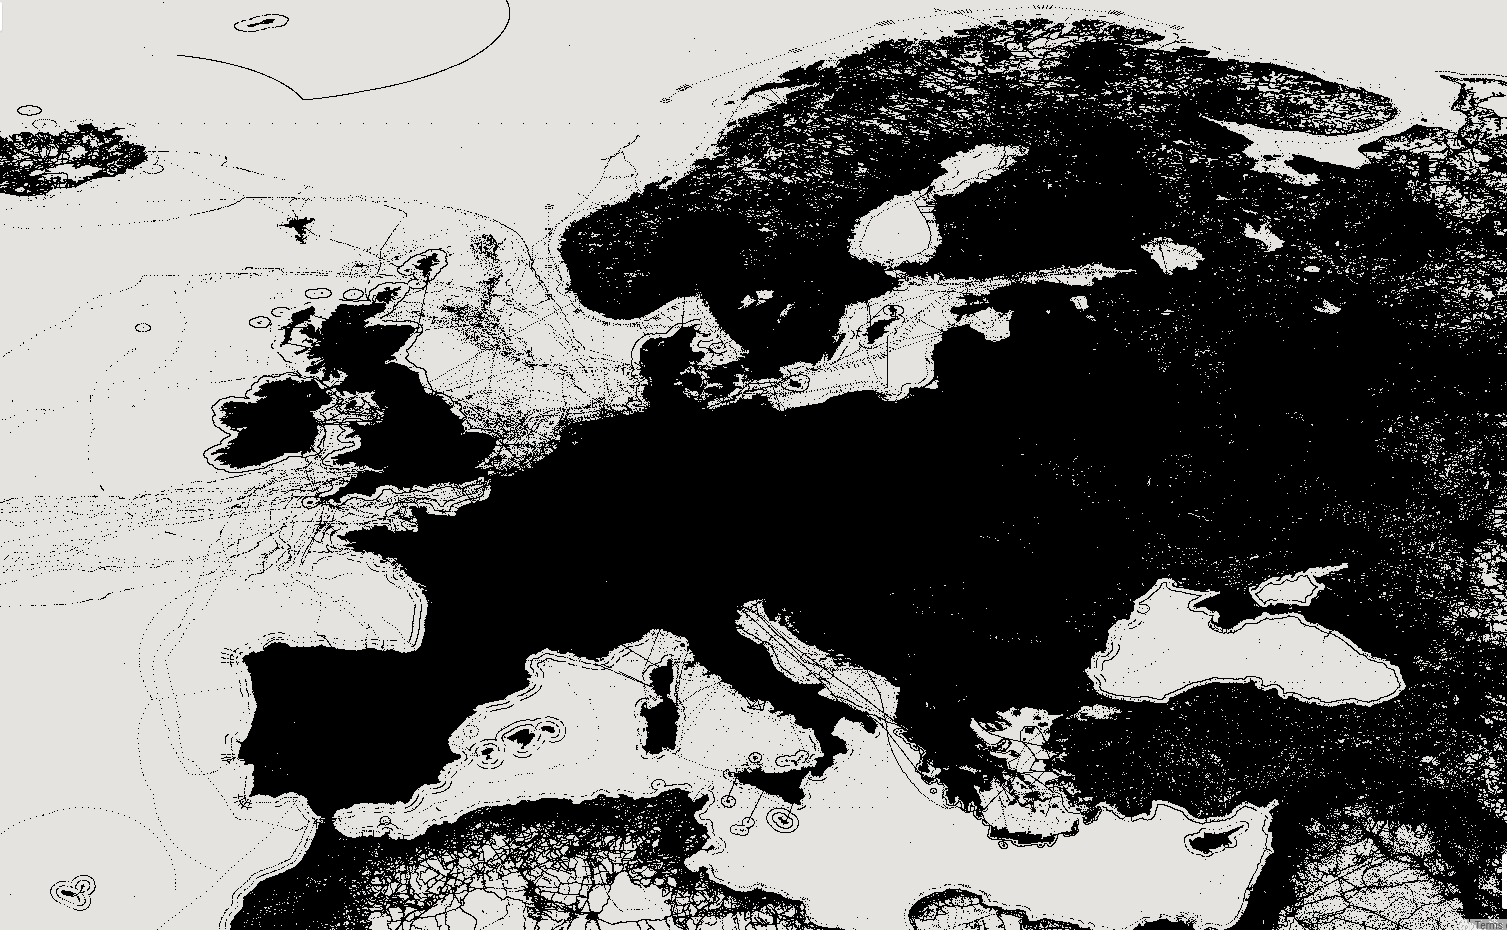
\includegraphics[width=1\textwidth]{./img/motivace/eu_all.png}
		\end{frame}
	
		\begin{frame}
			\frametitle{Vizualizace 1.3 miliardy bodů po prostorové agregaci}
			\centering
			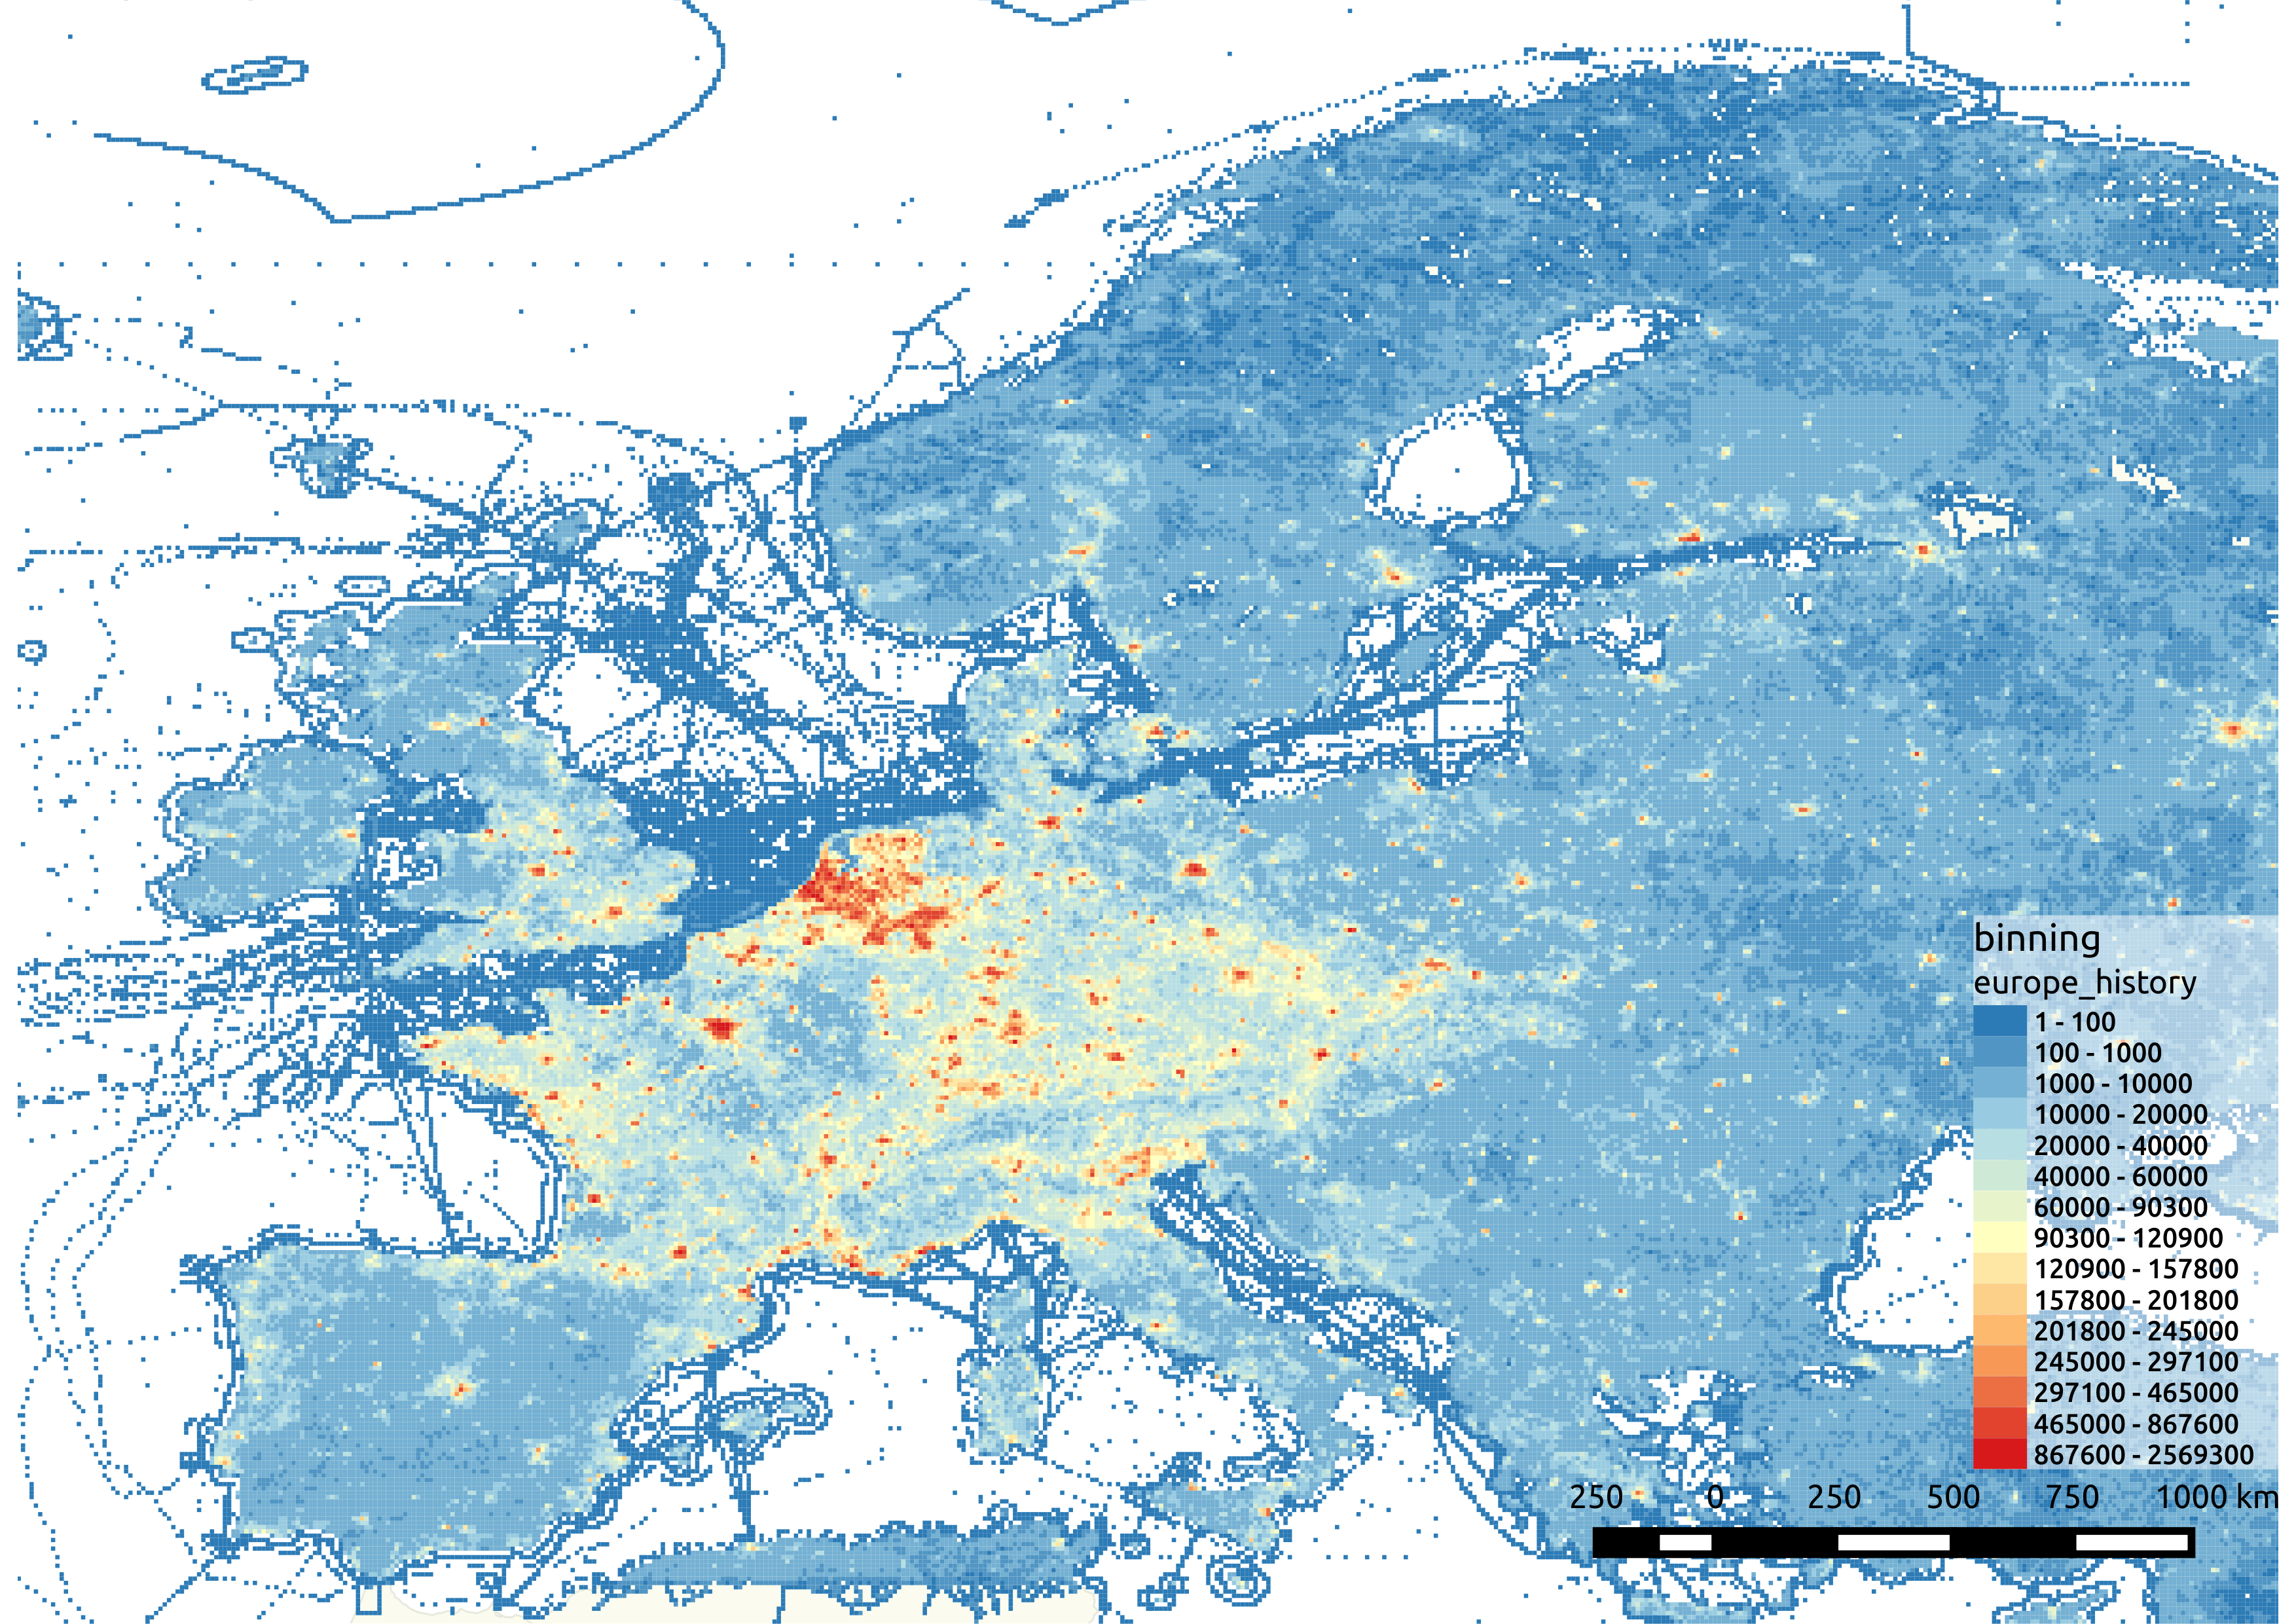
\includegraphics[width=1\textwidth]{./img/spatial/history.png}
		\end{frame}
	
	\section{Závěr}
	\subsection{Výsledky práce}		
	\begin{frame}
		\frametitle{Závěr}
		Výsledky práce:
		\begin{enumerate}
			\item  Vysvětlení teoretických principů distribuované databáze Hadoop
				\begin{itemize}
					\item Hadoop Distributed File System
					\item MapReduce
				\end{itemize}
			\item Úvod do problematiky GIS extenzí pro Hadoop
				\begin{itemize}
					\item Analýza teoretických aspektů
					\item Porovnání dostupných GIS extenzí pro Hadoop
				\end{itemize}
			\item Využití cloud služby Google Cloud Platform
				\begin{itemize}
					\item Konfigurace projektu
					\item Konfigurace Hadoop clusteru
				\end{itemize}
			\item Implementace vlastních nástrojů pro GRASS GIS
				\begin{itemize}
					\item Umožnění využití Hadoop GIS extenzí z desktop GIS
				\end{itemize}
		\end{enumerate}
	\end{frame}
	
	\subsection{Navazující práce}	
	\begin{frame}
		\frametitle{Navazující práce}
		Navazující práce:
		\begin{itemize}
			\item Návrh knihoven systematicky implementuje core API nezávisle na GRASSu = možnost implementace Hadoop frameworku pro QGIS bez zásahů do těchto knihoven. Je třeba dopsat pouze konverzi map, která je v QGIS také založena na OGR driveru + implemenace GUI pro QGIS. 
			
			\item Implementace podpory Oozie workflow pro plánování Hadoop úloh.  
		\end{itemize}
	\end{frame}
	
	\begin{frame}
	\centering
	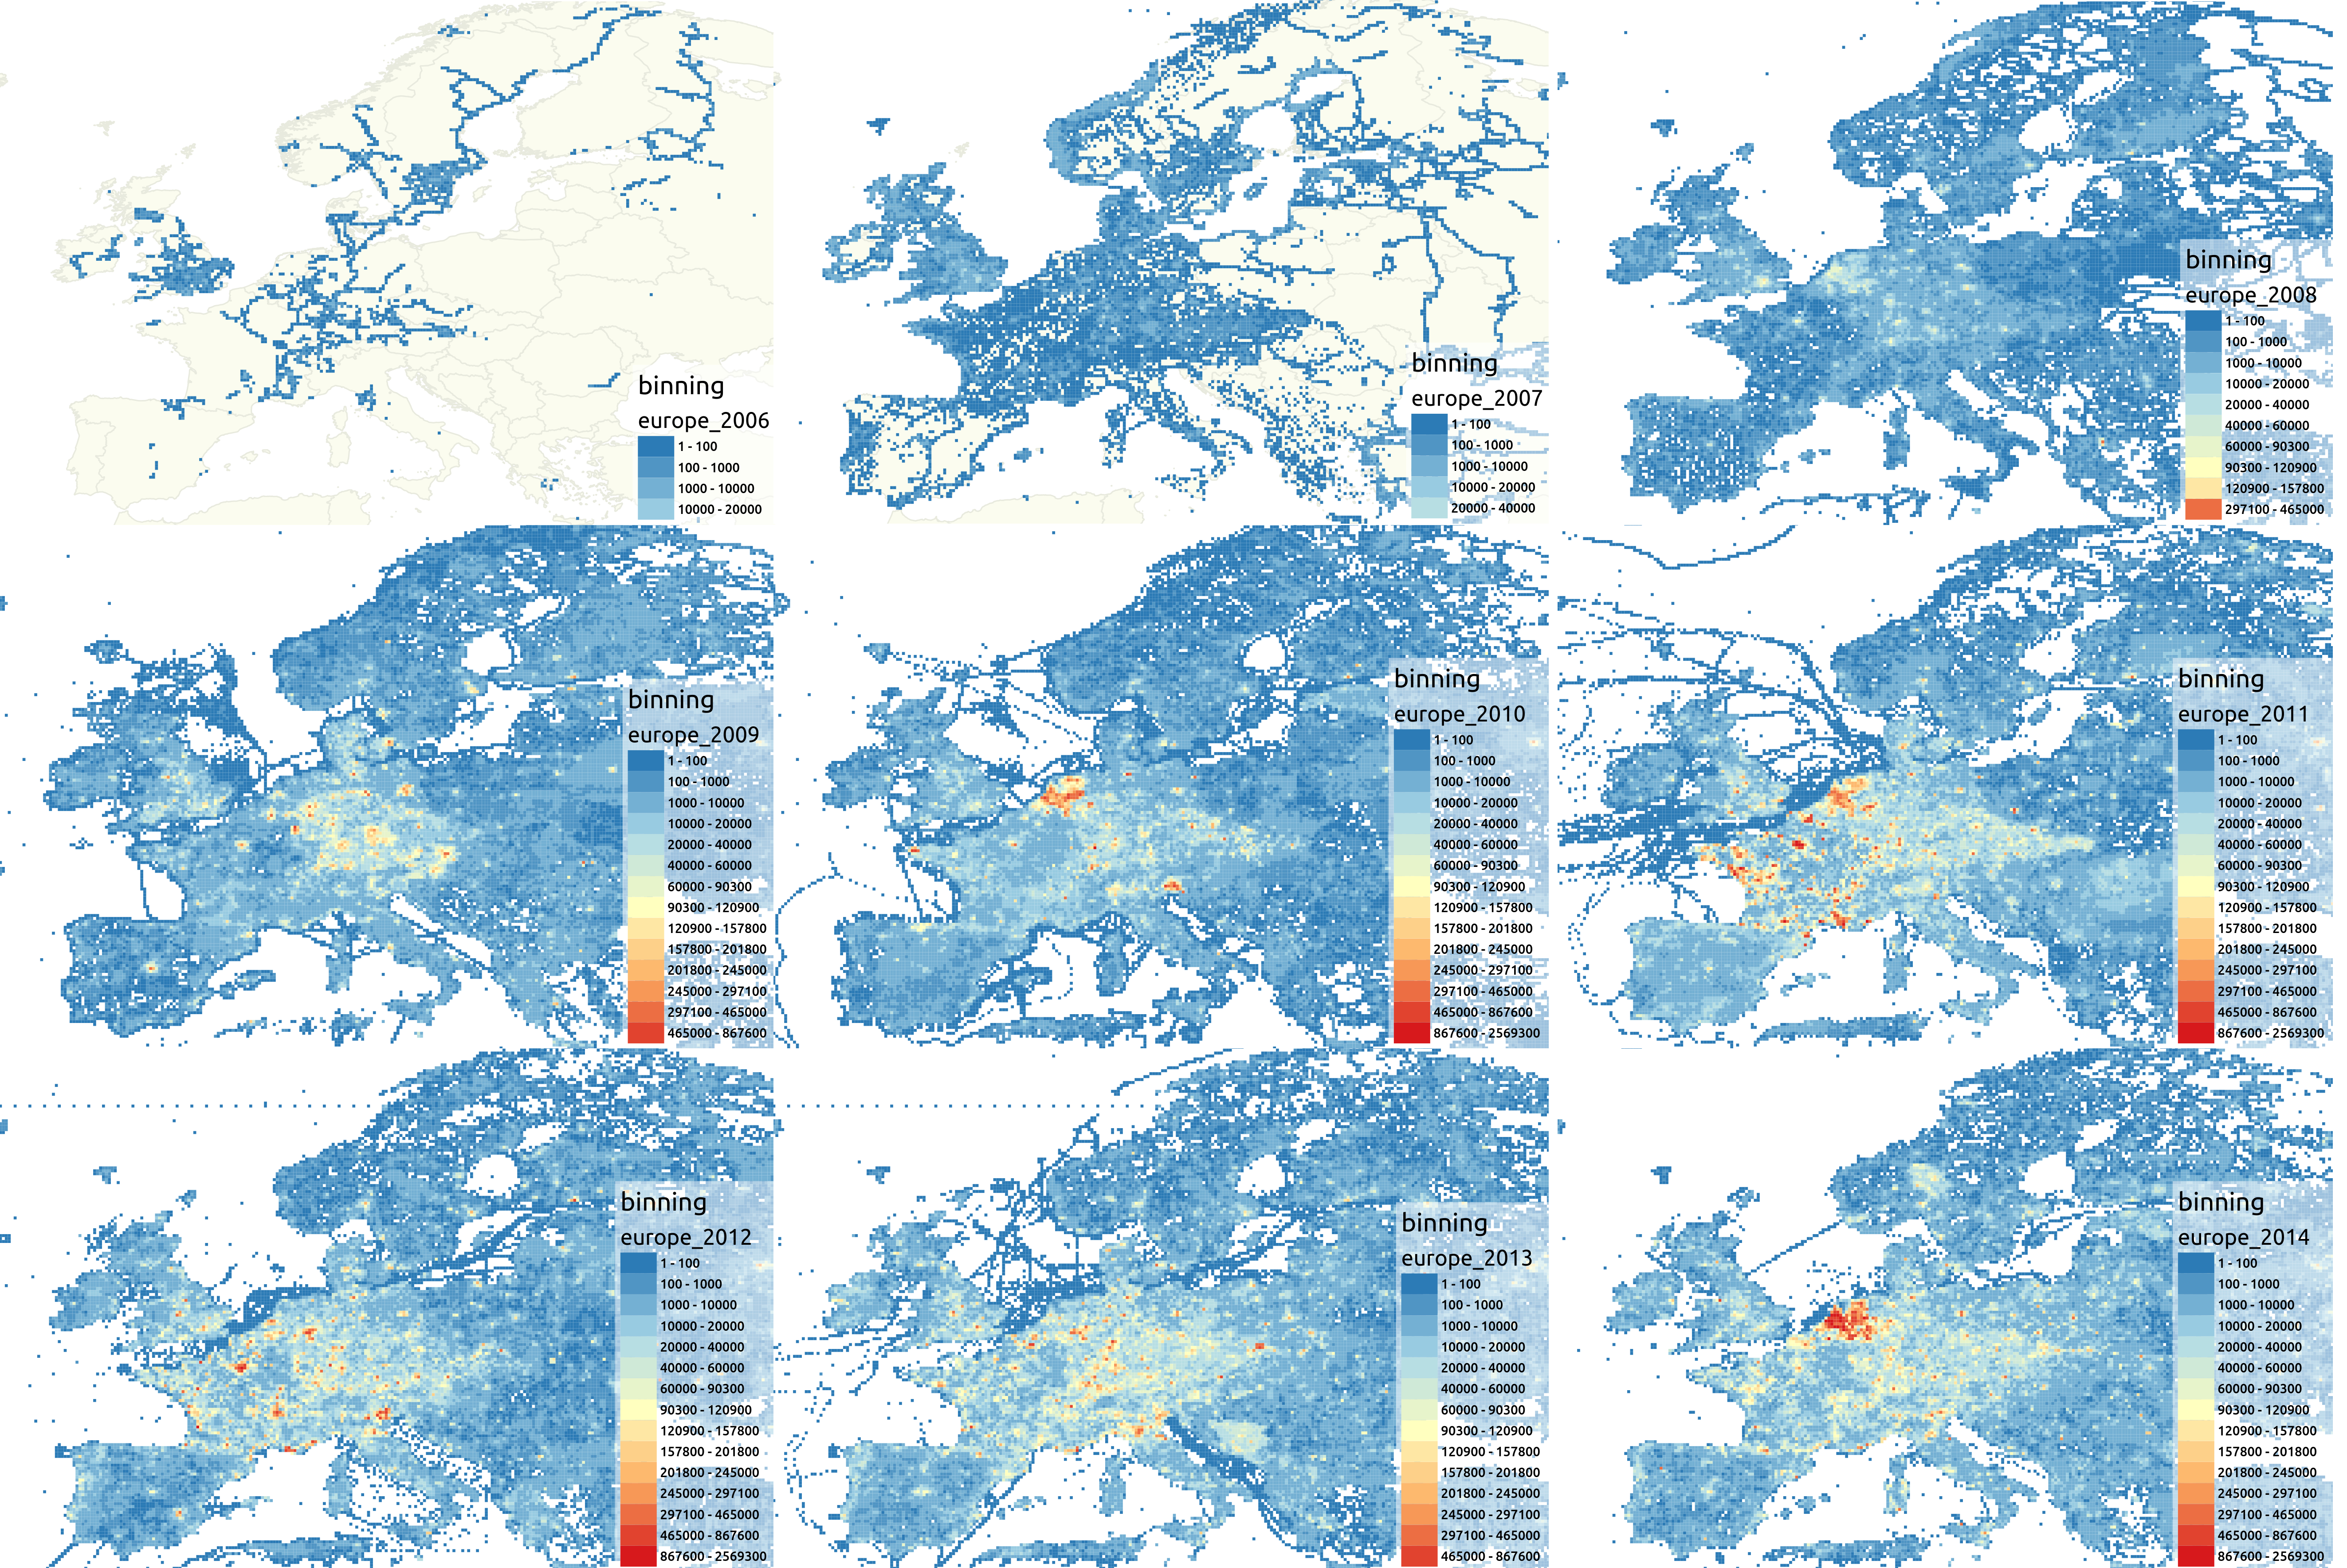
\includegraphics[width=1\textwidth]{./img/osm/merge.png}
	
	\Huge Děkuji za pozornost
	\end{frame}
	
	
	
	
	\section{Otázky oponenta}
	\begin{frame}
		\frametitle{Reakce na poznámky oponenta}
		\small
		\begin{enumerate}
			\item Jaké další frameworky typu Hadoop existují?
			\begin{itemize}
			\item Spark
			\item MongoDB
			\end{itemize}

			\pause[]  
			
			\item Pokud je možné Hadoop provozovat na Google cloudu, jaké jsou další cloud možnosti? 
						Např:
						\begin{itemize}
							\item BigQuery (Příloha A)
							\item Docker load balancing
						\end{itemize}
									%Google Cloud je stale rozvijejici se platforma, ktera umoznuje nespocet servisu. V priloze A jsem se zabival BigQuery- skalovatelna databaze
									%Dale mimo dp jsem zkousel vyuzit load balanceru  pro docker image obsahujici web. Umoznuje atomaticke skalovani v reakci na navstevnost a ze statistik navstevnosti
						 Jaké další cloud computing services diplomant zná?
 						\begin{itemize}
 							\item Amazoon Cloud
 							\item Docker Cloud
 						\end{itemize}
							%Dale znam Amazoon platformu a DockerCloud platformu, ktera je primo zavisla na Amazoon a umoznuje maintenance Docker konteinteru
							Proč zvolil právě Hadoop?
							%Hadoop jsem zvolil jelikoz je nejrozsirenejsi platformou ve sfere distribuovanych databazi. A take proto, ze pro nej jsou dostupne GIS frameworky
						\begin{itemize}
							\item Nejrozšířenější platforma
							\item a proto nejširší dostupnost GIS nadstaveb
						\end{itemize}
								\end{enumerate}
							\end{frame}
	\section{Otázky oponenta}
	\begin{frame}
		\frametitle{Reakce na poznámky oponenta}
		

		\begin{enumerate}
					     \setcounter{enumi}{2}
			\item Výhody a nevýhody NoSQL databází vs "typické" relační databáze.
			
						Výhody NoSQL 
						\begin{itemize}
							\item Komoditní hardware
							\item Škálování do šířky
							\item Vysoká dostupnost (replikace)
							\item Uložení nestrukuralizovaných dat
							\item Dynamické přidávaní dat
						\end{itemize}
						
						Výhody SQL
					\begin{itemize}
						\item Normalizace 
						\item Relační schémata - lepší orientace v db
						\item Datové typy, validace
						\item Klíče
						\item SQL standard
						\item Striktní transakce - izolace
					\end{itemize}
		%Vyhody NoSQL
			%potreba vykoneho hardware a i presto narazi na limity pro ukladani velkeho objemu dat
			%skalovani do sirky pro nosql X vertikalni pro RDBMS 
			%Vysoka dostupnost dostupne -replikace, faul tolerant
			%Rychla odezva i pro velka data
			%Linearni skalovani - do sirky
			%ulozeni nestrukturovanych dat
			%dynamicke pridavani dat(v pripade alter table je tabulka offline)
		%Nevyhody
			%
		\end{enumerate}
	\end{frame}
	


	
	
	
	
	
\end{document}

